% !TEX root = monografia.tex
\chapter{Desenvolvimento}
Neste capítulo será abordado o processo de desenvolvimento do aplicativo \textit{Android}, do sistema de cadastramento, do \textit{web service} e o banco de dados utilizado.

\section{\textit{Beacon}}
Foram utilizados três \textit{beacons} da marca \textit{Estimote} para realização dos testes.

Estes \textit{Beacons} são pequenos dispositivos com a configuração de \textit{32-bit ARM® Cortex CPU} acompanham acelerômetro, sensor de temperatura e, o mais importante, \textit{bluetooth 4.0 Smart}, também conhecido como \textit{bluetooth de baixa energia}. Eles possuem um alcance máximo aproximado de 70 metros, porém, devido a interferências, em um contexto real estima-se entre 40-50 metros.\cite{estimote}

Eles possuem informações que são úteis para programar e identificar cada \textit{beacon}.

\textbf{\textit{UUID}}: É uma \textit{string} de 16 byte que é utilizada para diferenciar um grupo grande de \textit{beacons}. No caso do Infobeacons foi aplicado o mesmo \textit{UUID} para todos os \textit{beacons}.

\textbf{\textit{Major}}: É uma \textit{string} de 2 bytes que é usada para distinguir um grupo menor de \textit{beacons}.

\textbf{\textit{Minor}}: É uma \textit{string} de 2 bytes que é usada para identificar um único \textit{beacon} dentro do grupo.

\textbf{\textit{MAC}}: É uma \textit{string} de 6 bytes utilizada como endereço físico para comunicação com a interface de rede.

\textbf{\textit{TxPower}}: É empregado como mensurador da distância do dispositivo com relação ao \textit{beacon}. Ele é calibrado com a distância equivalente a um metro.

Ao permacener com emissão constante de sinal \textit{bluetooth} é possível identificar as informações acima para que sejam utilizadas no desenvolvimento.

\section{\textit{Bluetooth 4.0}}
O \textit{bluetooth} é uma tecnologia que faz a conexão de dispositivos eletrônicos entre si, através de ondas de rádio, sem o uso de cabos ou fios, necessitando apenas da aproximação dos dispositivos. Essa tecnologia trás consigo a liberdade do contato com aparelhos residenciais como, ouvir música pelo chuveiro, controlar sua TV e até mesmo ascender as luzes da casa através de seu \textit{smartphone} ou \textit{tablet} \cite{bluetooth}.

A ideia de criar o \textit{bluetooth} veio da companhia Ericsson que ao longo do tempo atraiu outras companhias como a Intel, IBM, Toshiba e Nokia entre outras que com o passar dos anos também aderiram a esse consórcio. A diversidade de companhias colaborou com o desenvolvimento dessa tecnologia para reconhecimento nos vários tipos de dispositivos \cite{alecrim}.

Como a evolução da tecnologia é constante, a versão 4.0 do \textit{bluetooth} traz consigo seu benefício, economia de energia, caso o aparelho esteja com o \textit{bluetooth} ativo, mas sem ser utilizado por um tempo, ele entra em economia de energia até que volte a ser usado. 

\section{\textit{Android}}
Foi escolhido o \textit{Android} como linguagem principal, pois a maioria dos aparelhos em nosso meio possuem o \textit{Android} como sistema operacional e pelo fato de ter maior acessibilidade para ser desenvolvido.

De acordo com a \textit{Kantar World Panel}, a venda de \textit{Smartphones Android} no Brasil em Janeiro de 2016 possuía a porcentagem de 92,4\% com relação aos outros Sistemas operacionais. \cite{kantar}

\begin{figure}[H]
  \centering
  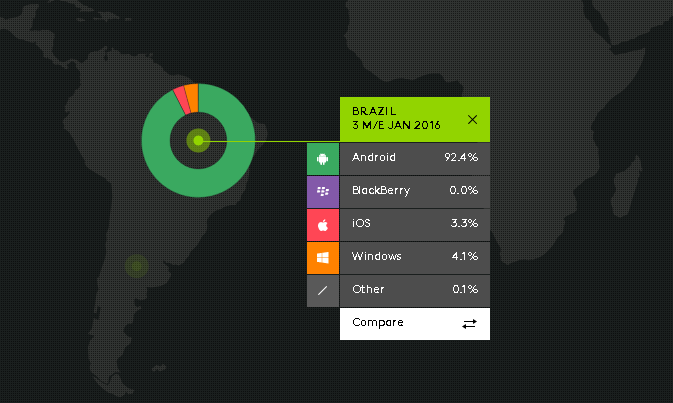
\includegraphics[width=13cm]{./figs/porcentagem_android.png}
  \caption{Sistemas Operacionais \textit{Mobile} no Brasil}
  \par\makebox[\width]{Fonte: Autores}
\end{figure}

\section{\textit{TalkBack}}

\textit{TalkBack} não é uma coisa que você vai querer utilizar ao menos que você precise dele.

Pessoas que têm dificuldade em ver a sobrecarga de informação que um \textit{smartphone} moderno tem para oferecer pois precisam de alguma ajuda. A \textit{Google} fornece um conjunto muito abrangente de ferramentas de respostas. \textit{Google TalkBack} é um serviço de acessibilidade que auxilia deficientes visuais e usuários com baixa visão a interagir e usufruir de seus dispositivos.
Ele converte os textos em voz, emite vibrações e é possível saber o que pode ser feito conforme o toque na tela. É um serviço integrado com o \textit{Android}, pois já vem instalado com o sistema operacional. \cite{talkback}

Ele funciona da seguinte maneira: o usuário utiliza os dedos para explorar a tela do dispositivo até o momento que atinja algum elemento ou texto. Logo, ao identificar este elemento, o \textit{TalkBack} se encarregará de converter em voz sua informação. Esta informação pode ser uma mensagem, um texto ou até a etiqueta de conteúdo do elemento.

Segundo a Google \cite{etiquetas} ''Os utilizadores de serviços de acessibilidade, como leitores de ecrã, recorrem a etiquetas de conteúdo para compreender o significado dos elementos numa interface.

Em alguns casos, como quando as informações são transmitidas graficamente num elemento, as etiquetas de conteúdo podem fornecer uma descrição de texto do significado ou da ação associada ao elemento.

Se os elementos numa interface do utilizador não fornecerem etiquetas de conteúdo, pode ser difícil para alguns utilizadores compreender as informações apresentadas ou efetuar ações na interface''.

\subsection{Gestos e Navegação}
A priori, os gestos e a navegação do \textit{TalkBack} pode ser complicado para quem possui boa visão, pois não é um recurso essencial para a navegação no Sistema Operacional do dispositivo. Contudo, existem usuários que necessitam deste recurso de acessibilidade para que seja possível navegar e utilizá-lo de forma plena no dia a dia.

Desta forma, eles precisam aprender alguns gestos para usufruir de todas as funcionalidades proposta pelo Sistema Operacional.

Segue alguns exemplos de gestos disponibilizados pela Google.

\begin{table}[H]
    \centering
    \begin{tabular}{|l|l|}
        \hline
        \textbf{Ação} & \textbf{Gesto} \\ 
        \hline
        Mover para o próximo item na tela & Deslizar para a direita \\
        \hline
        Mover para o item anterior na tela & Deslizar para a esquerda \\
        \hline
        Percorrer as configurações de navegação	& Deslizar para cima ou para baixo \\
        \hline
        Selecionar item em foco & Tocar duas vezes\\
        \hline
    \end{tabular}
    \caption{Gestos básicos}
    \label{tab:gestos_basicos}
\end{table}

\begin{table}[H]
    \centering
    \begin{tabular}{|p{7cm}|p{7cm}|}
        \hline
        \textbf{Ação} & \textbf{Gesto} \\ 
        \hline
        Mover para o primeiro item na tela & Para cima e para baixo \\
        \hline
        Mover para último item na tela & Para baixo e depois para cima \\
        \hline
        Rolar para a frente
(se estiver em uma página maior que a tela) & Para a direita e depois para a esquerda \\
        \hline
        Rolar para trás
(se estiver em uma página maior que a tela) & Para a esquerda e depois para a direita \\
        \hline
        Mover controle deslizante para cima
(por exemplo, o volume) & Para a direita e depois para a esquerda \\
        \hline
        Mover controle deslizante para baixo
(por exemplo, o volume) & Para a esquerda e depois para a direita \\
        \hline
    \end{tabular}
    \caption{Gestos vai-e-vem}
    \label{tab:gestos_vaievem}
\end{table}

\begin{table}[H]
    \centering
    \begin{tabular}{|p{7cm}|p{7cm}|}
        \hline
        \textbf{Ação} & \textbf{Gesto} \\ 
        \hline
        Botão ''Início'' & Para cima e para a esquerda \\
        \hline
        Botão ''Voltar'' & Para baixo e para a esquerda \\
        \hline
        Apps recentes & Para a esquerda e para cima \\
        \hline
        Notificações & Para a direita e para baixo 
(veja a observação abaixo) \\
        \hline
        Abrir menu de contexto local & Para cima e para a direita \\
        \hline
        Abrir menu de contexto global & Para baixo e para a direita \\
        \hline
    \end{tabular}
    \caption{Gestos angulados}
    \label{tab:gestos_angulados}
\end{table}

\subsection{Como ativar o \textit{TalkBack}}

Para que seja ativado o \textit{TalkBack} no \textit{Android} o usuário deve seguir os seguintes passos:

Passo 1: Entrar nas ''Configurações'' do dispositivo, selecionar a opção ''Acessibilidade'' e depois clicar em ''\textit{TalkBack}''.

\begin{figure}[H]
  \centering
  \subfloat[Configurações]{\label{talkback1}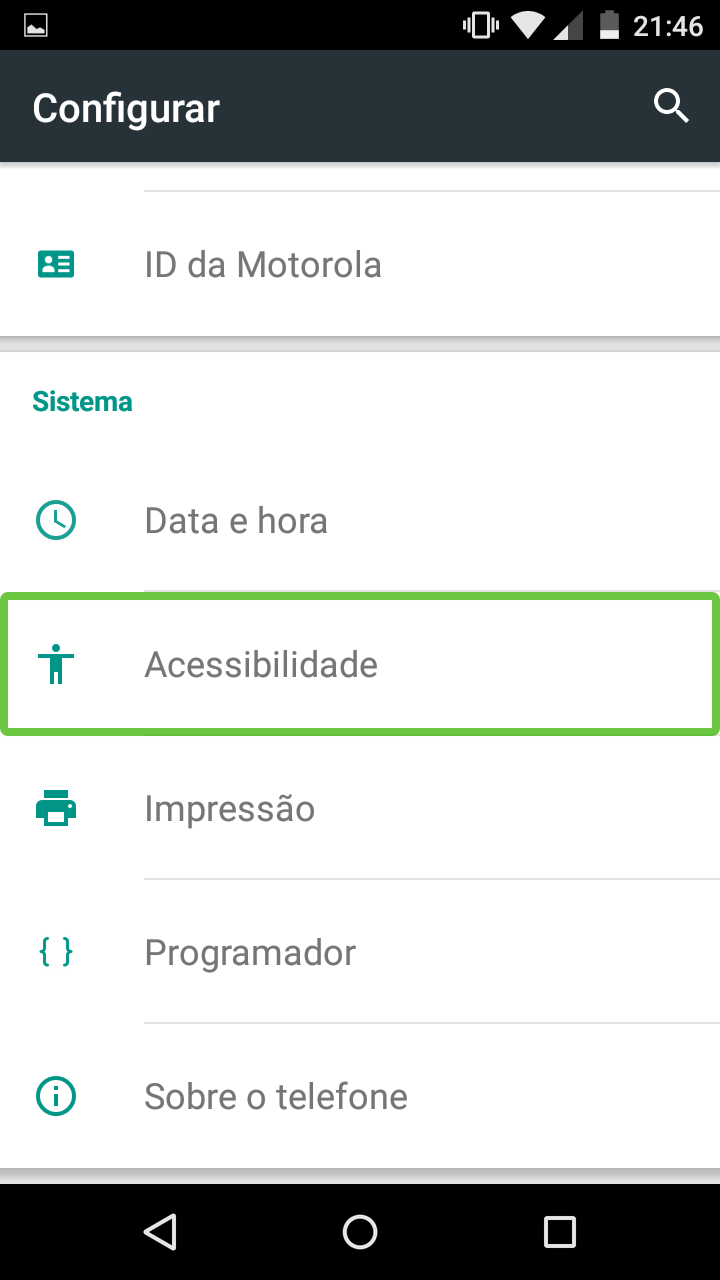
\includegraphics[width=4.7cm]{./figs/talkback2.png}}
  \subfloat[Acessibilidade]{\label{talkback3}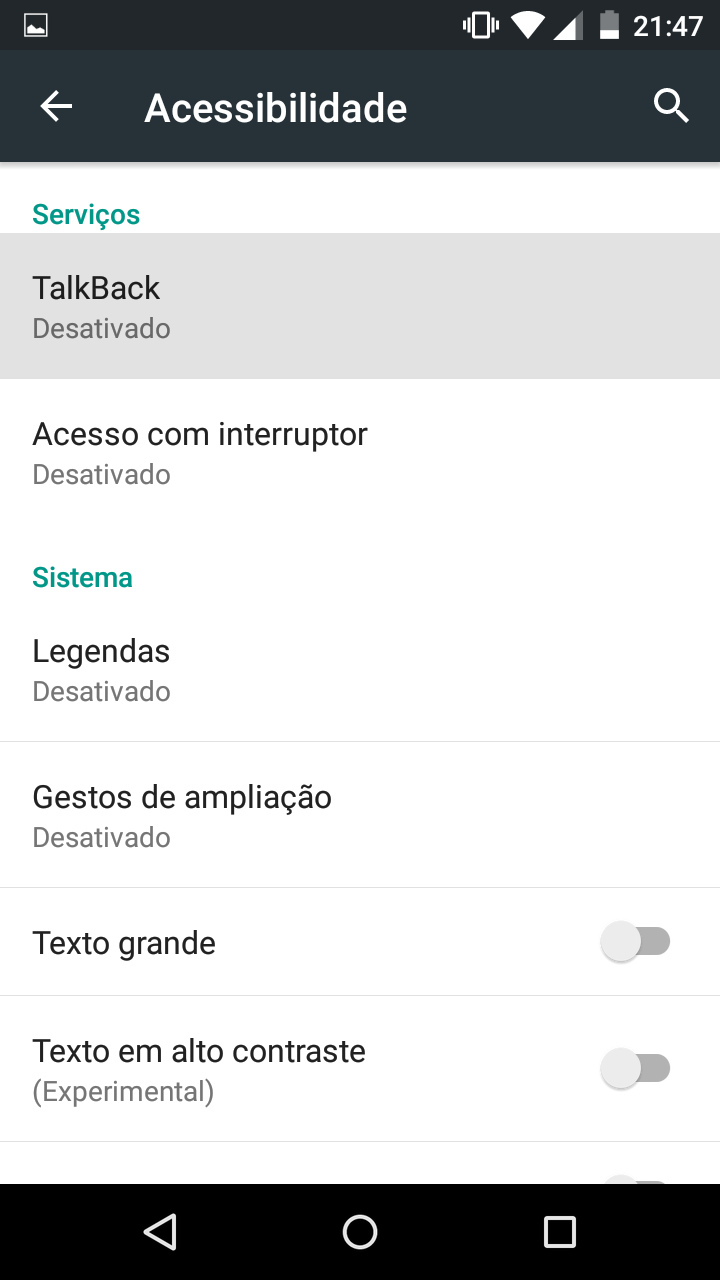
\includegraphics[width=4.7cm]{./figs/talkback3.png}}
  \caption{\label{talkback6}Configurações}
  \par\makebox[\width]{Fonte: Autores}
\end{figure}

\begin{figure}[H]
  \centering
  \subfloat[\textit{TalkBack}]{\label{talkback4}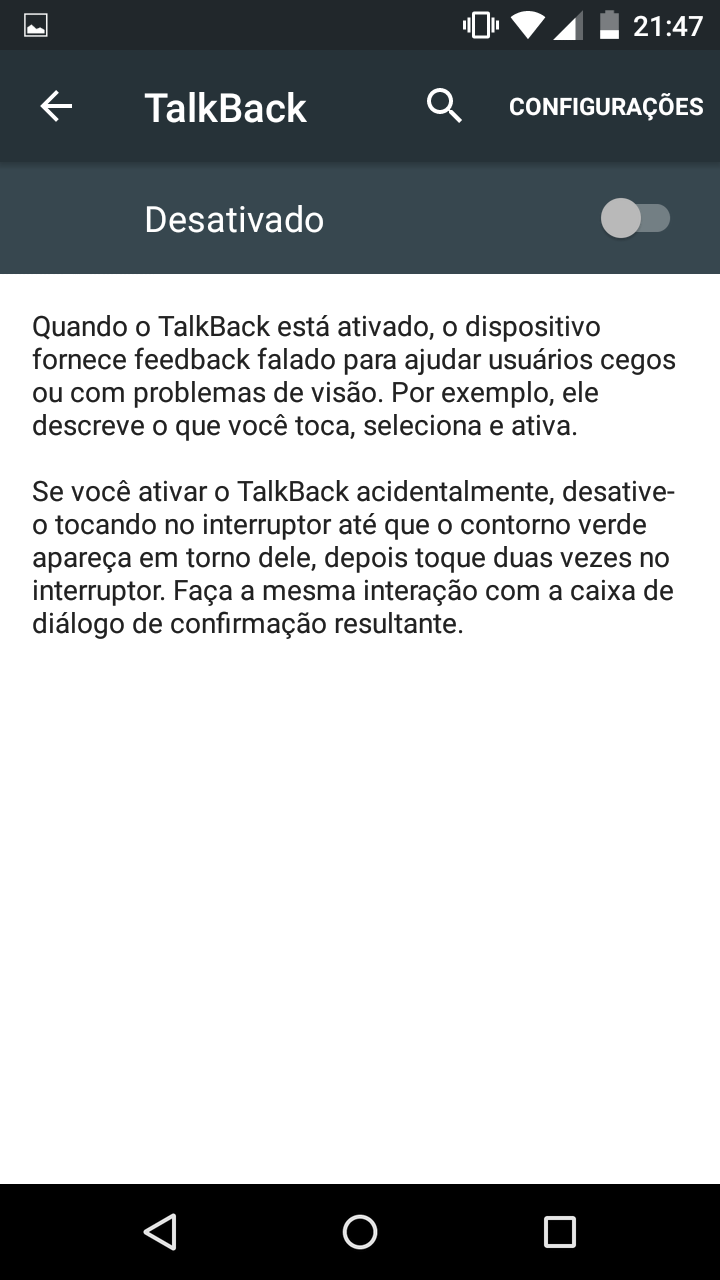
\includegraphics[width=4.7cm]{./figs/talkback4.png}}
  \subfloat[Ativar]{\label{talkback5}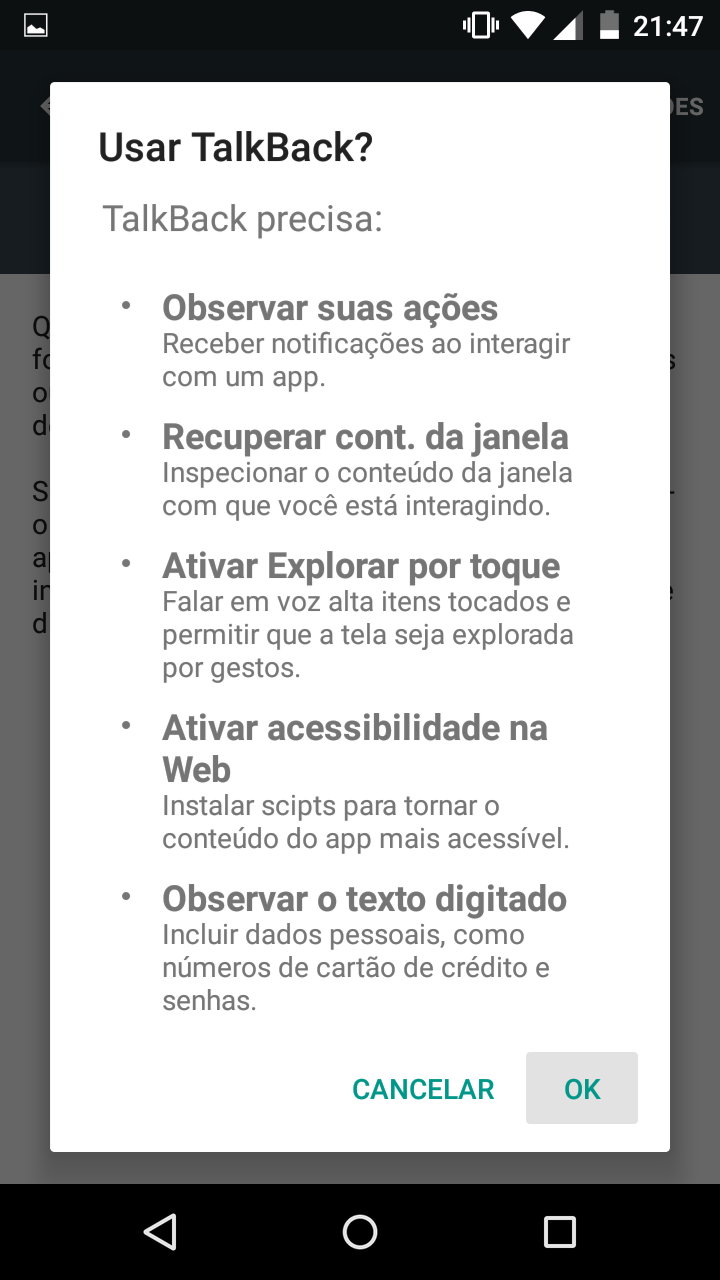
\includegraphics[width=4.7cm]{./figs/talkback5.png}}
  \caption{\label{talkback2}Ativação \textit{talkback}}
  \par\makebox[\width]{Fonte: Autores}
\end{figure}

Passo 2: Clicar no \textit{Switch} para ativar. Será aberta um alerta com as permissões necessárias para o funcionamento do \textit{TalkBack}.

Passo 3: Clicar em ''OK''.

\subsection{Como desativar o \textit{TalkBack}}

Para desativar o \textit{TalkBack} é necessário acessar novamente a opção \textit{TalkBack} do menu de acessibilidade e clicar no elemento presente na parte superior direita da tela (mesma opção utilizada para a ativação). Logo, será exibida uma mensagem de confirmação para parar o \textit{TalkBack} e clicando em ''Ok'' ele será desativado.

\begin{figure}[H]
  \centering
  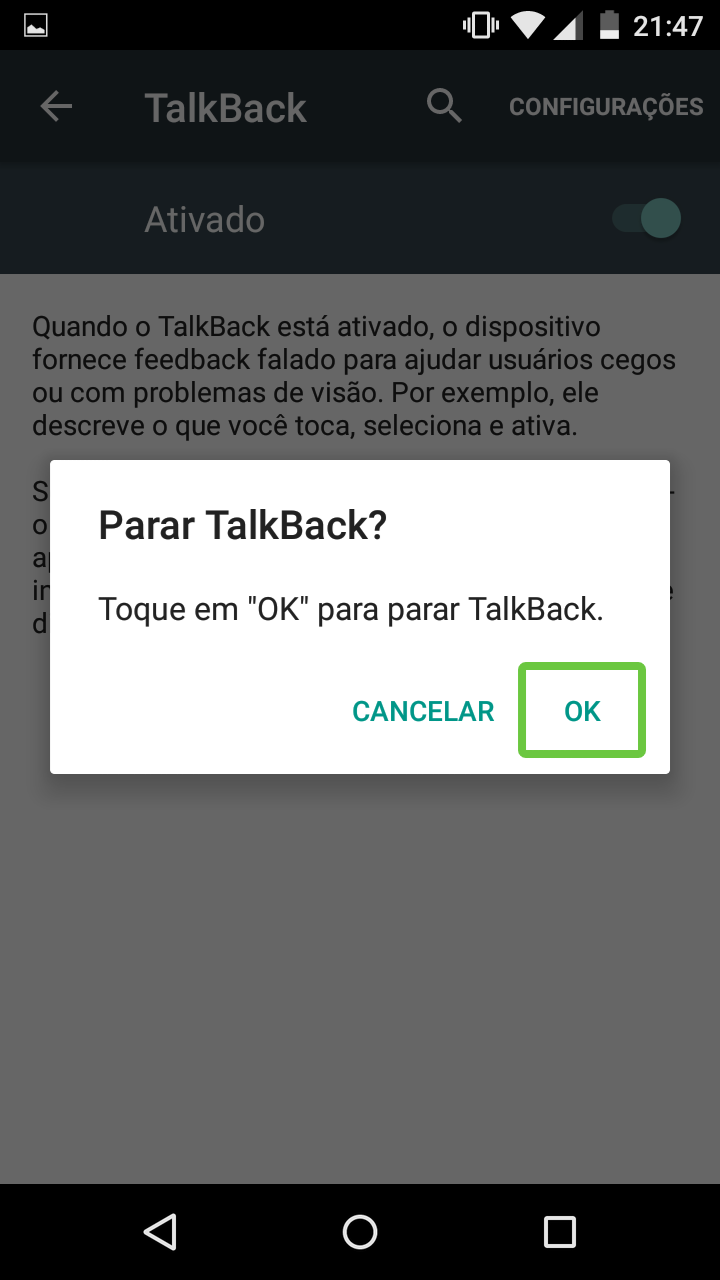
\includegraphics[width=4.7cm]{./figs/desativar_talkback.png}
  \caption{Desativar \textit{TalkBack}}
  \par\makebox[\width]{Fonte: Autores}  
\end{figure}

\section{Desenvolvendo o aplicativo Infobeacons}
O aplicativo foi desenvolvido em \textit{Android}, utilizando o \textit{Android Studio 2.0} como ferramenta. Ao abrir o aplicativo é apresentada a \textit{splash screen} com o logo do \textit{Infobeacons} e só dará lugar a tela seguinte quando o processamento dela estiver completo. 

\textit{Splash Screen} é uma tela inicial que, geralmente, possui o logo do aplicativo ou uma imagem e pode conter também uma barra de progresso. A função dela é referente a usabilidade do usuário quanto ao carregamento do aplicativo, pois permanece ativa enquanto é carregada a próxima tela e é destruída ao final deste carregamento. Desta forma, o usuário fica ciente que as informações estão sendo carregadas.

\begin{figure}[H]
  \centering
  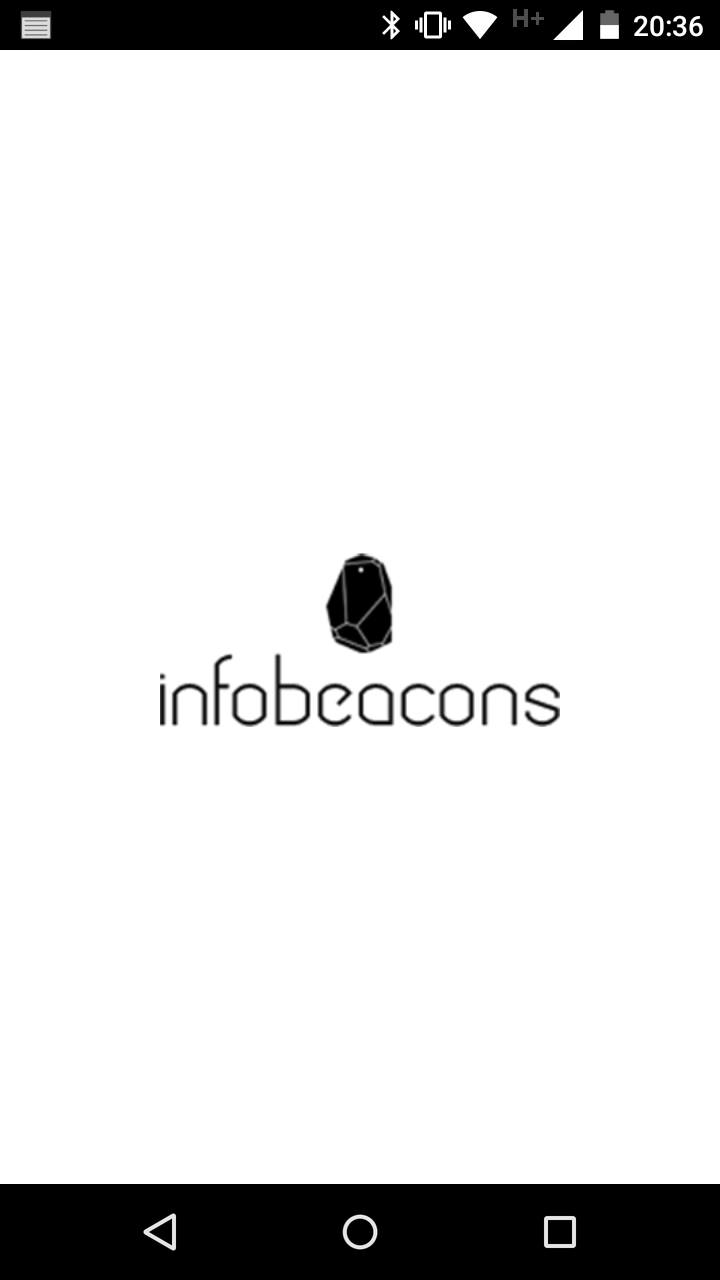
\includegraphics[width=4.7cm]{./figs/app1.png}
  \caption{Splash Screen}
  \par\makebox[\width]{Fonte: Autores}
\end{figure}

Antes de começar a procurar os \textit{beacons} se faz necessária a ativação do \textit{bluetooth} e uma conexão ativa com a internet, seja por \textit{Wi-Fi} ou \textit{3G/4G}.

\textbf{\textit{Bluetooth}}: É por meio do \textit{bluetooth} que o dispositivo \textit{Android} realiza o reconhecimento dos \textit{beacons} e recebe as informações dele.

\textbf{Internet}: Possui o papel de realizar requisições \textit{HTTP} no \textit{web service} e recuperar informações lá cadastradas para o \textit{beacon} cujo endereço físico foi passado como parâmetro da requisição.

Mediante ao \textit{bluetooth} estar desativado ao iniciar o aplicativo, será exibida uma \textit{pop-up} solicitando a permissão para que o \textit{bluetooth} seja ativado pelo próprio aplicativo. Ao clicar na opção ''permitir'' será iniciada a busca pelos \textit{beacons} normalmente, no entanto, caso seja escolhida a opção ''recusar'' o aplicativo exibirá um alerta em forma de \textit{toast} informando que deverá ser ativado o \textit{bluetooth} para que funcione corretamente.

\textbf{\textit{Toast}}: Alerta nativo do \textit{Android} que é exibido na parte inferior da tela e possui certa duração entre aparecer e desaparecer. A duração pode ser curta ou longa e ele é captado pelo \textit{TalkBack} assim que é exibido.

Se o dispositivo não possuir conexão ativa com a internet enquanto o aplicativo está aberto, a qualquer momento pode ser exibido um alerta em forma de \textit{toast} com a informação de que é necessária conexão com internet para o funcionamento correto.

Ambos são exemplificados pelas figuras abaixo.

\begin{figure}[H]
  \centering
  \subfloat[Permissão \textit{Bluetooth}]{\label{bluetooth}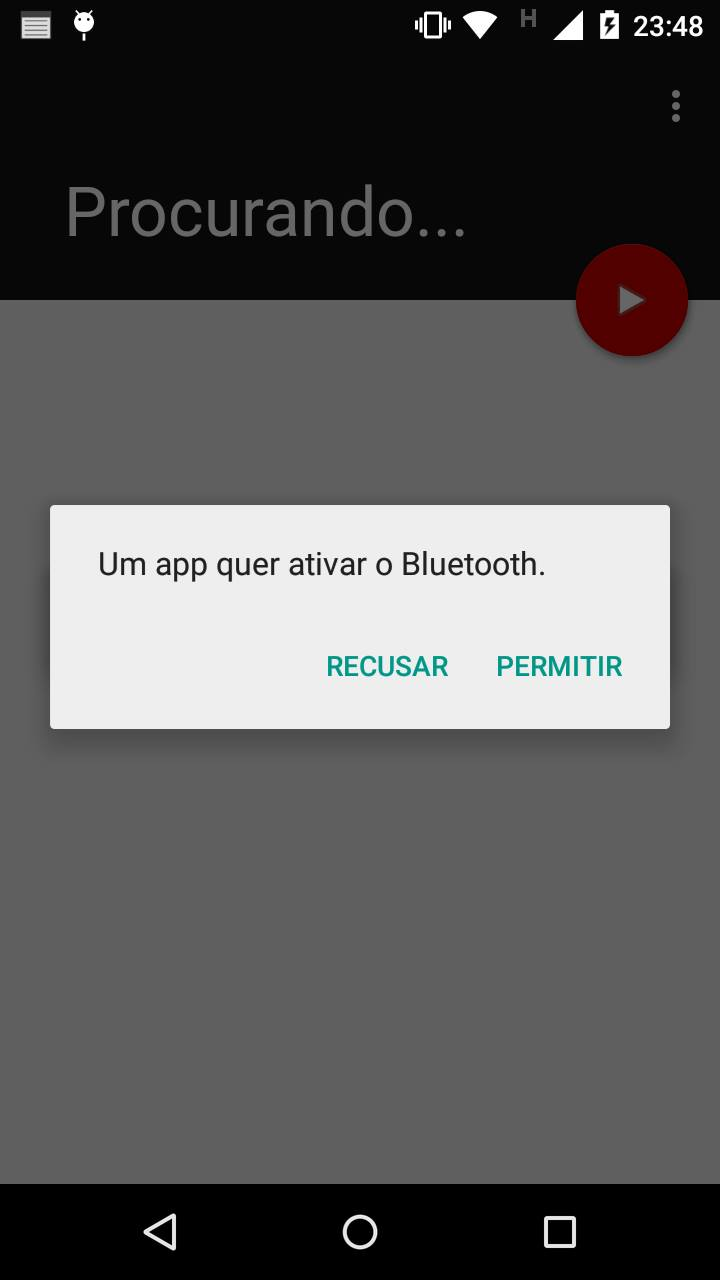
\includegraphics[width=4.7cm]{./figs/app6.png}}
  \subfloat[Internet]{\label{internet}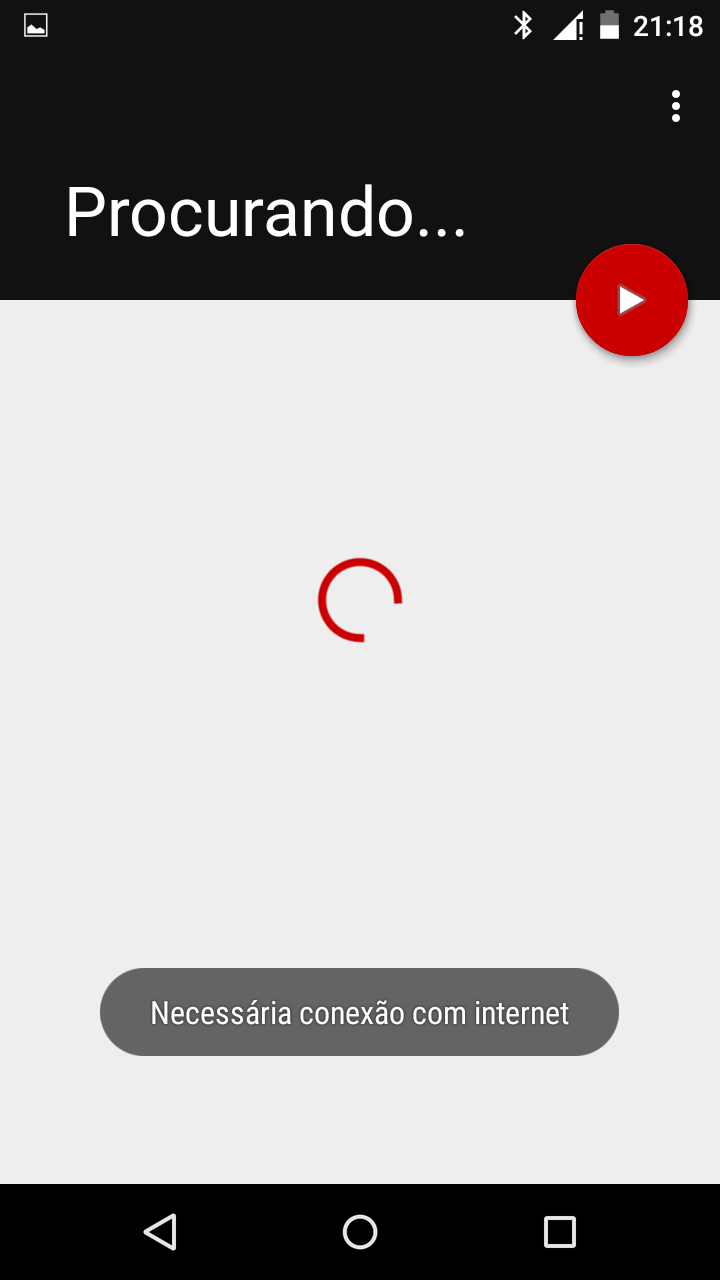
\includegraphics[width=4.7cm]{./figs/Internet.png}}
  \caption{\label{internet_bluetooth}Permissões}
  \par\makebox[\width]{Fonte: Autores}
\end{figure}

\begin{figure}[H]
  \centering
  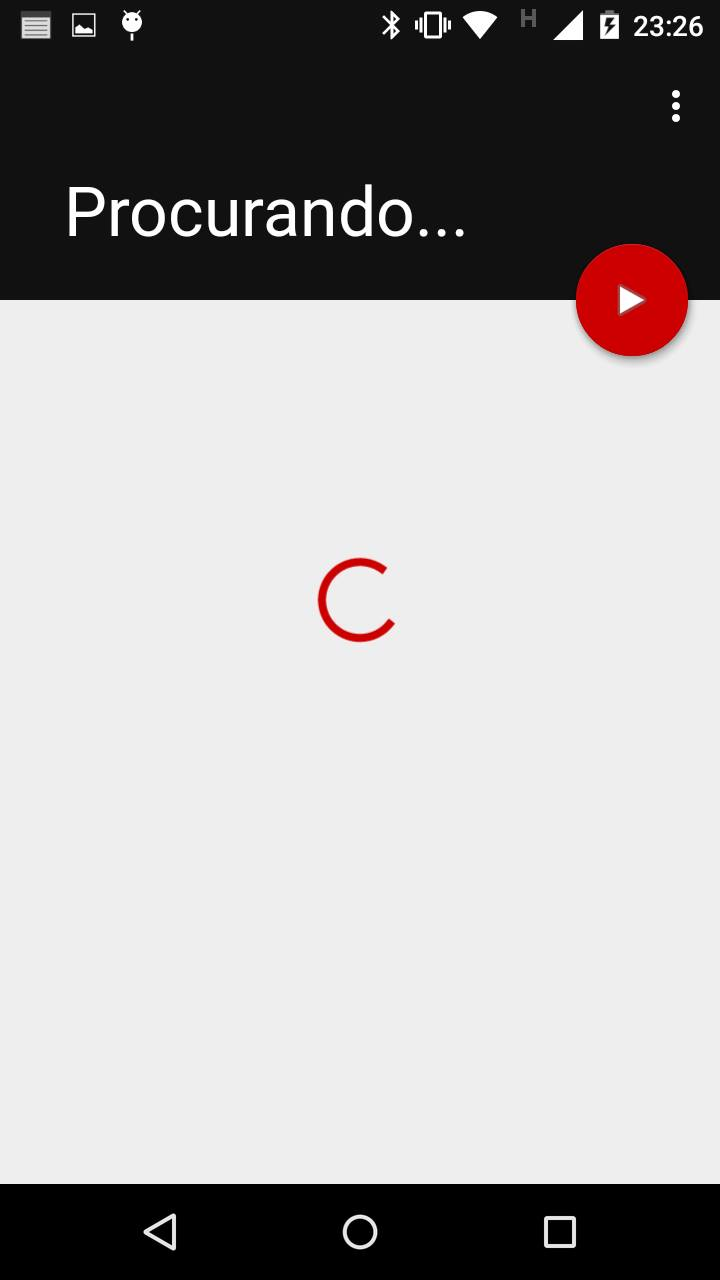
\includegraphics[width=4.7cm]{./figs/app2.png}
  \caption{Procurando}
  \par\makebox[\width]{Fonte: Autores}
\end{figure}

Neste momento, com conexão a internet e com \textit{bluetooth} ativado, o aplicativo começa a fazer a verificação dos \textit{beacons} ao seu redor. Será permanecida a busca até o momento que seja detectado algum \textit{beacon} próximo, independente se o usuário estiver parado ou estar em movimento.

Existe um elemento gráfico, nativo do \textit{Android}, localizado no centro da tela que fica em constante rotação indicando que o aplicativo está buscando os \textit{beacons}.

Ao realizar o reconhecimento do \textit{beacon} mais próximo são recebidas todas as informações dele tais como \textit{UUID}, \textit{Major}, \textit{Minor}, \textit{MAC}, dentre outras. 

O dado mais importante e essencial neste cenário é o endereço \textit{MAC}. Ele será adicionado como parâmetro em uma \textit{URL}, será feita uma requisição \textit{HTTP} por meio desta \textit{URL}, chegará a um método no \textit{web service} que buscará as informações cadastradas no banco de dados para aquele determinado \textit{beacon} e será retornado um \textit{JSON} para o aplicativo.

Ao realizar a requisição com sucesso e obter este retorno do objeto \textit{JSON} o aplicativo organizará estas informações na tela do dispositivo da seguinte forma:

\textbf{Barra superior}: Alterada para o nome do \textit{beacon} recebido pela requisição.

\textbf{Abaixo da barra superior}: Painel de imagem que exibirá a imagem recebida pela requisição.

\textbf{Abaixo da imagem}: Exibição do texto referente ao conteúdo recebido pela requisição.

É apresentada uma mensagem em forma de \textit{toast} informando que os dados foram encontrados, pois ela será lida pelo \textit{TalkBack} do dispositivo caso ele esteja ativo.

No entanto, se ocorrer alguma falha na requisição \textit{HTTP} será exibida na tela a mensagem ''[Erro] Tentando novamente...'' e o aplicativo fará outra tentativa.

\begin{figure}[H]
  \centering
  \subfloat[Permissão \textit{Bluetooth}]{\label{bluetooth23}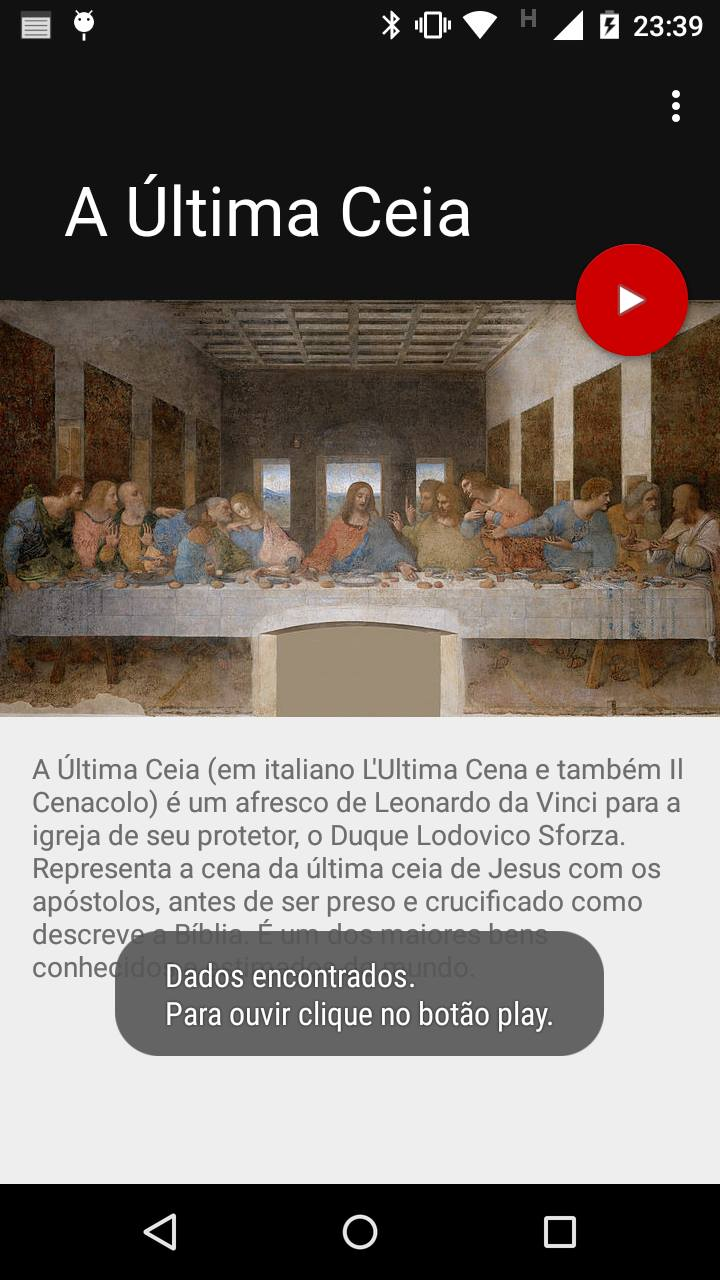
\includegraphics[width=4.7cm]{./figs/app3.png}}
  \subfloat[Internet]{\label{internet42}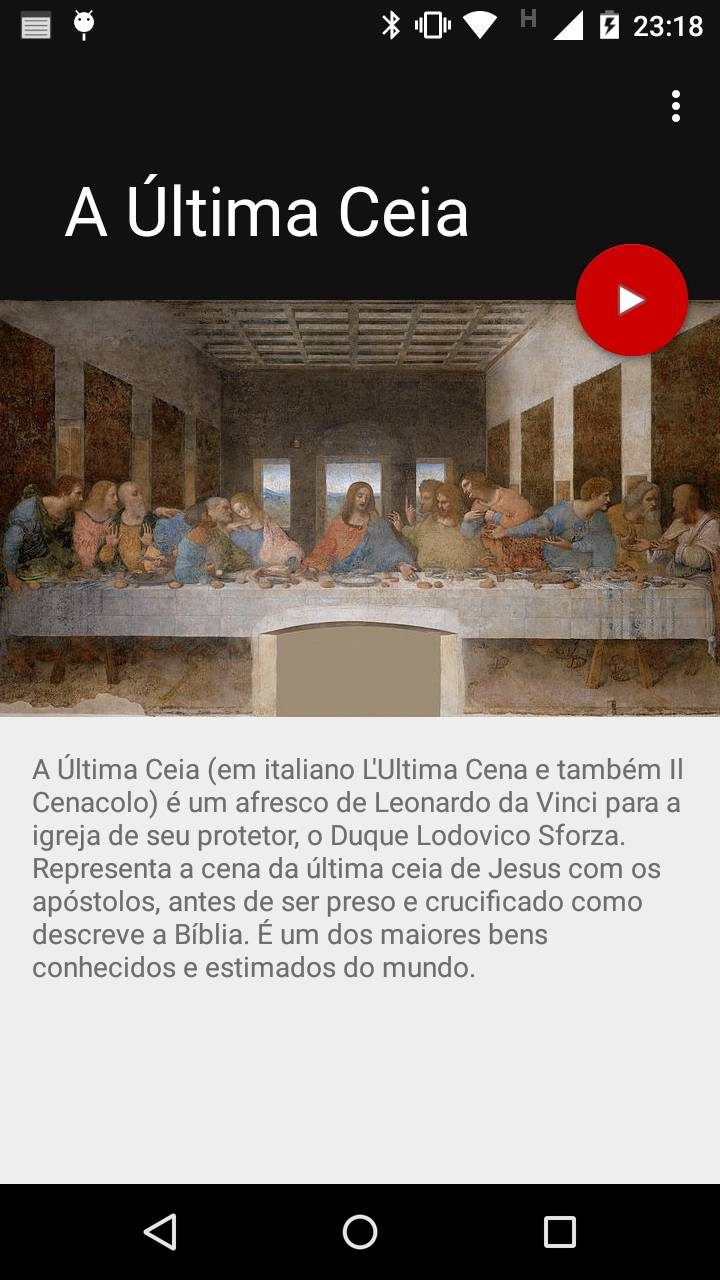
\includegraphics[width=4.7cm]{./figs/app4.png}}
  \caption{\label{internet_bluetooth_permissoes}Permissões}
  \par\makebox[\width]{Fonte: Autores}
\end{figure}

A partir do momento que a informação está carregada na tela, o usuário consegue visualizar as informações ali descritas. Se o texto for muito extenso para caber na tela do dispositivo, é possível utilizar o gesto de \textit{scroll} para ir rolando o texto conforme a leitura.

Foi criado um botão de play localizado na parte superior direita para que usuários em geral possam ouvir o texto referente ao \textit{beacon}. 

Este botão possui etiqueta de identificação para os usuários de \textit{TalkBack} e, quando acionado, converte o texto exibido na tela em voz através do \textit{Text to Speech}.

\textbf{\textit{Text to Speech}}: É uma biblioteca nativa do \textit{Android} responsável por converter o texto em voz.

Para auxiliar os usuários foi criado um painel de ajuda acessado pela opção localizada no canto superior direito.
Este painel contém as informações sobre os requisitos para que o aplicativo funcione corretamente e uma breve explicação.

\begin{figure}[H]
  \centering
  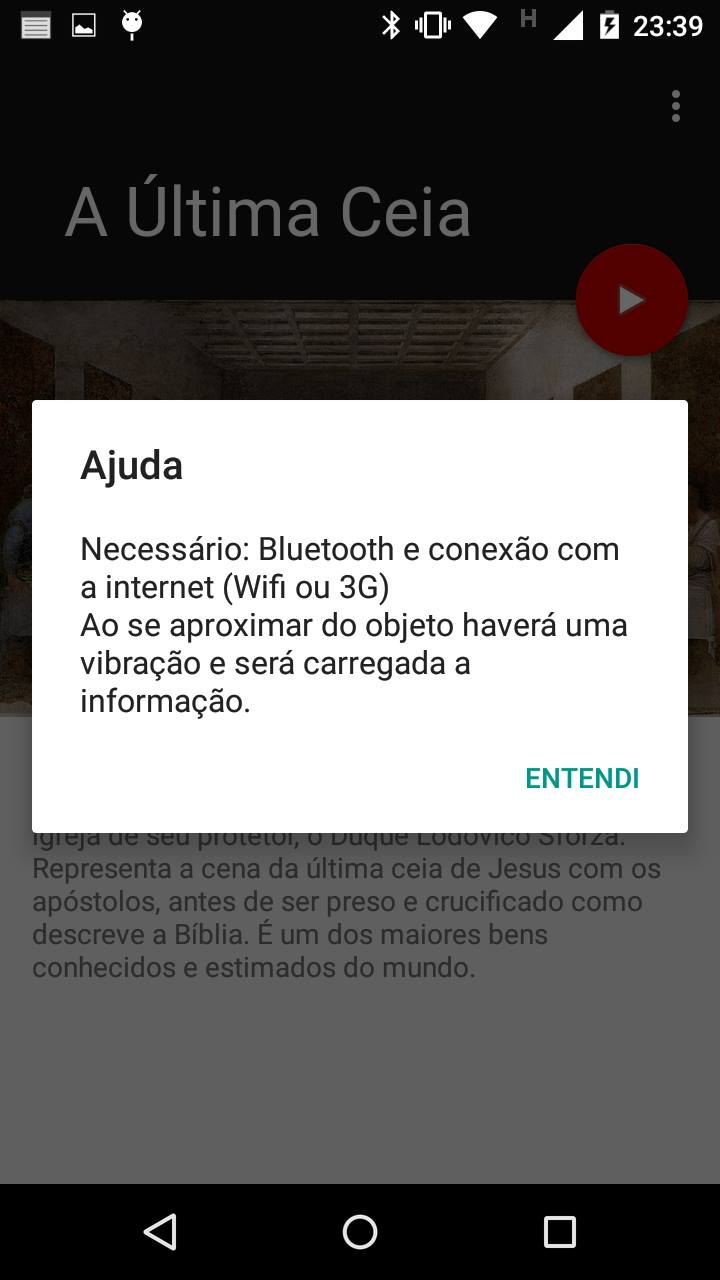
\includegraphics[width=4.7cm]{./figs/app5.png}
  \caption{Painel de ajuda}
  \par\makebox[\width]{Fonte: Autores}
\end{figure}

\subsection{\textit{Android Studio} 2.0}
Para o desenvolvimento na linguagem \textit{Android} foi utilizado o \textit{Android Studio} 2.0.
O \textit{Android Studio} é o ambiente de desenvolvimento integrado (\textit{IDE}) oficial para o desenvolvimento de aplicativos \textit{Android} e é baseado no \textit{IntelliJ IDEA}. \cite{androidstudio}

\begin{figure}[H]
  \centering
  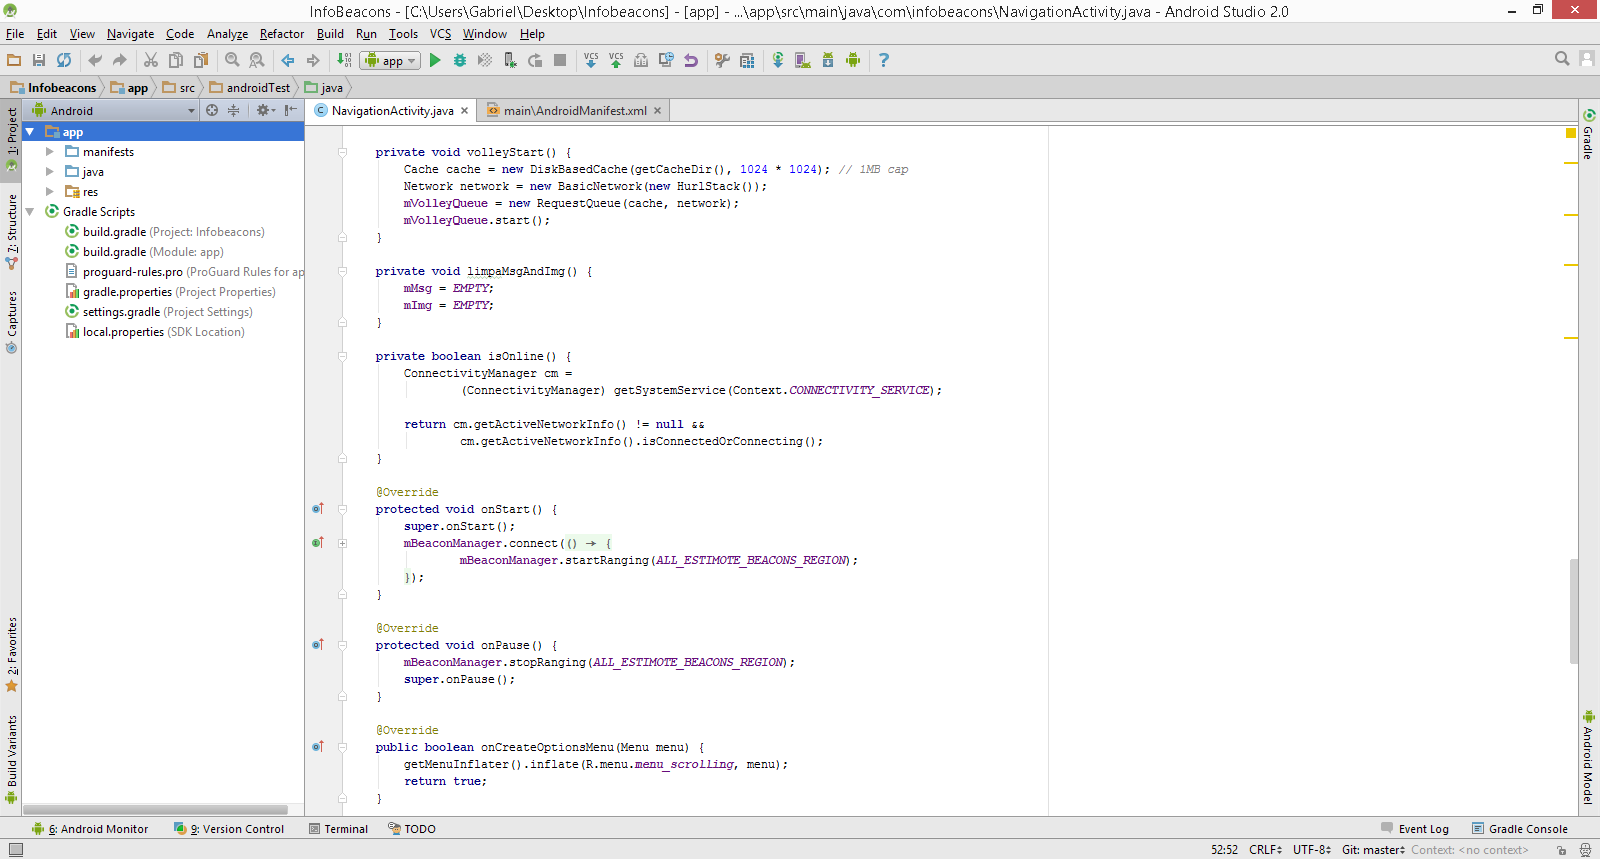
\includegraphics[width=14cm]{./figs/Android_Studio.png}
  \caption{Desenvolvimento \textit{Android} Studio}
  \par\makebox[\width]{Fonte: Autores}
\end{figure}

\subsection{Aparelho \textit{Android}}
%Especificações do Dispositivo
Os \textit{Smartphones Android} utilizados para a realização dos testes do aplicativo foram:

\begin{table}[H]
    \centering
    \begin{tabular}{|p{7cm}|p{7cm}|}
        \hline
        \multicolumn{2}{|c|}{Especificações técnicas} \\ 
        \hline
        Marca & Motorola \\
        \hline
        Modelo & Moto G \\
        \hline
        Sistema Operacional & Android 5.1 Lollipop \\
        \hline
        Tamanho da tela & 4,5'' polegadas \\
        \hline
    \end{tabular}
    \caption{Moto G}
    \label{tab:phone1}
\end{table}

\begin{table}[H]
    \centering
    \begin{tabular}{|p{7cm}|p{7cm}|}
        \hline
        \multicolumn{2}{|c|}{Especificações técnicas} \\ 
        \hline
        Marca & Samsung\\
        \hline
        Modelo & Galaxy J7\\
        \hline
        Sistema Operacional & Android 6.0 Marshmallow\\
        \hline
        Tamanho da tela &  5,5'' polegadas\\
        \hline
    \end{tabular}
    \caption{Samsung Galaxy J7}
    \label{tab:phone2}
\end{table}

\section{Desenvolvendo o sistema de cadastramento de \textit{beacons}}

\subsection{Ferramentas}
O Eclipse versão Luna foi a principal \textit{IDE} utilizada para o desenvolvimento do sistema em \textit{Java}.

\subsection{Mapa mental do sistema de cadastramento de beacons}
O mapa mental representa as rotas do sistema de cadastramento de beacons, com todos os fluxos que podem ser seguidos nele.

\begin{figure}[H]
  \centering
  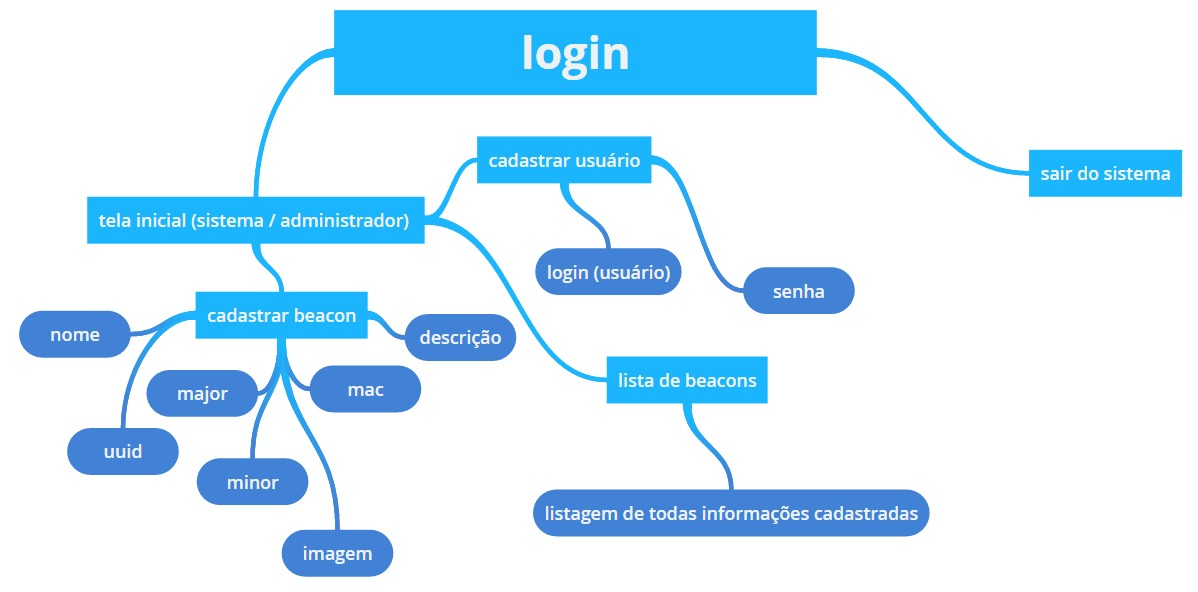
\includegraphics[width=13cm]{./figs/MapaMental.jpg}
  \caption{Mapa mental}
  \par\makebox[\width]{Fonte: Autores}
\end{figure}

\subsection{Telas}

A primeira tela do nosso sistema de cadastramento é um login. Por questões de segurança, o administrador principal do projeto deverá ter a conta criada pelo próprio desenvolvedor, com esse login em mãos ele poderá cadastrar novos usuários. 

Caso o usuário preencha os dados pedido pelo formulário erroneamente, os campos digitados serão apagados automaticamente e em seguida o mesmo deve preenchê-lo novamente.

\begin{figure}[H]
  \centering
  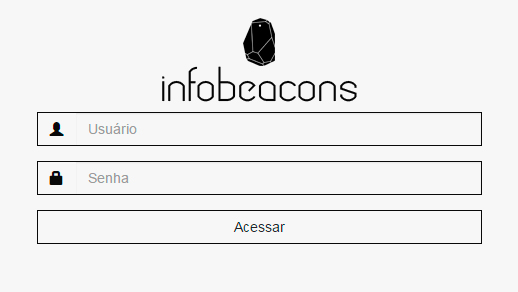
\includegraphics[width=12cm]{./figs/Login.jpg}
  \caption{Tela de login}
  \par\makebox[\width]{Fonte: Autores}
\end{figure}

Quando as informações forem devidamente cadastradas em seus respectivos \textit{beacons}, esta tela fará a listagem de todos esses objetos. Imagem, nome e \textit{MAC} serão referências para que o usuário identifique qual conteúdo ele cadastrou em determinado \textit{beacon}. 

O usuário ainda poderá executar algumas ações, como por exemplo excluir o \textit{beacon} ou apenas editá-lo. 

\begin{figure}[H]
  \centering
  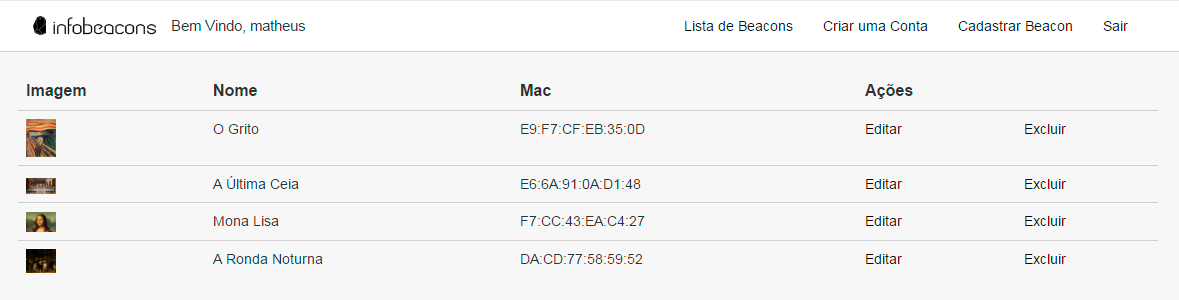
\includegraphics[width=16cm]{./figs/ListaBeacons.jpg}
  \caption{Tela de listagem de \textit{beacons}}
  \par\makebox[\width]{Fonte: Autores}
\end{figure}

\begin{figure}[H]
  \centering  
  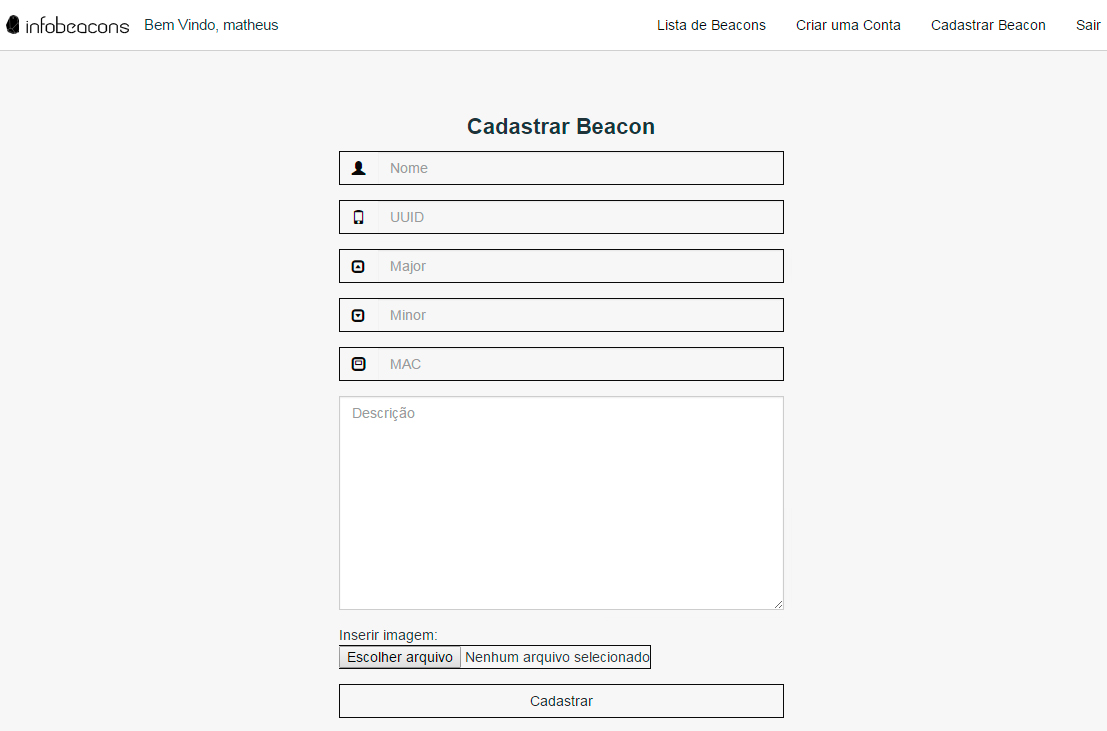
\includegraphics[width=14cm]{./figs/CadastrarBeacon.jpg}
  \caption{Tela de cadastrar \textit{beacons}}
  \par\makebox[\width]{Fonte: Autores}
\end{figure}

Os \textit{beacons} serão cadastrador de acordo com o que é pedido pelo formulário. Nome, \textit{UUID}, \textit{major}, \textit{minor} e \textit{MAC} são necessários para que o usuário tenha êxito neste processo. 

A imagem é o único campo que não é requerida, sendo assim, você pode terminar de cadastrar o \textit{beacon} normalmente, caso queira adicionar a imagem depois, basta entrar na tela de edição e subir uma imagem com até 300Kb. 

A tela de edição é exatamente igual a tela de cadastro, todas as informações cadastradas estará presente nela. Caso o usuário tenha escrito alguma palavra errada, adicionado a imagem errada ou até mesmo ter colocado alguma outra informação errada referente ao \textit{beacon}, ele poderá fazer as devidas correções.

\begin{figure}[H]
  \centering  
  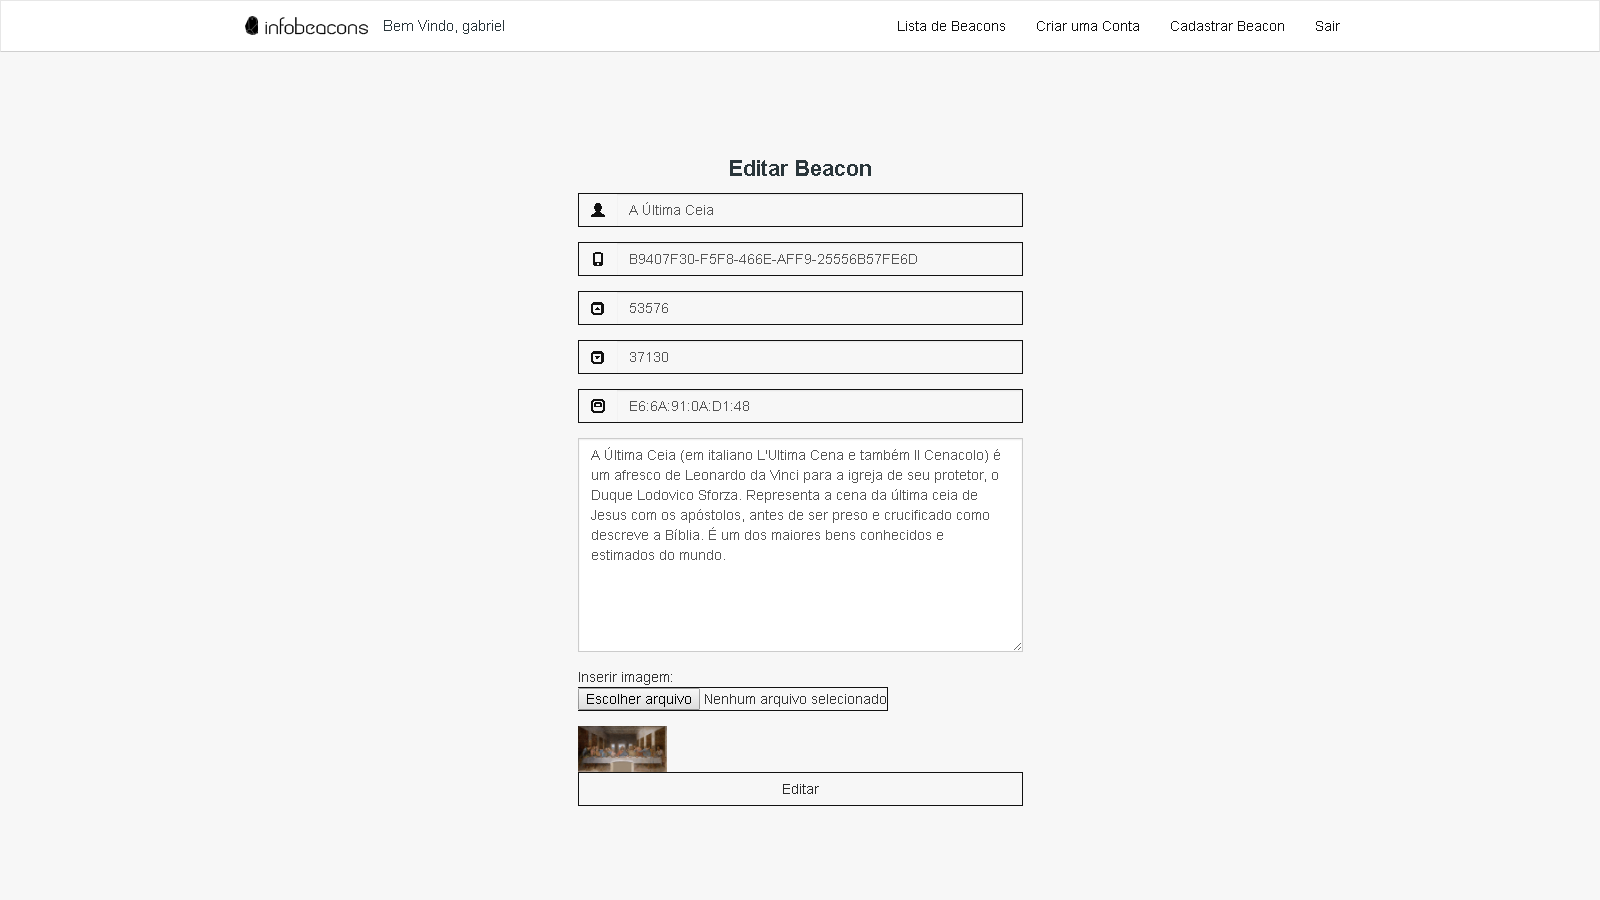
\includegraphics[width=16cm]{./figs/EditarBeacon.png}
  \caption{Tela de editar \textit{beacons}}
  \par\makebox[\width]{Fonte: Autores}
\end{figure}

\begin{figure}[H]
  \centering  
  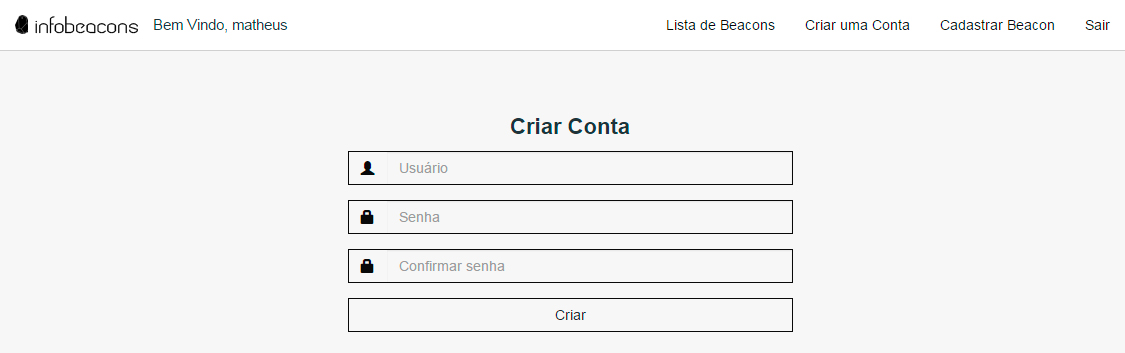
\includegraphics[width=16cm]{./figs/CriarConta.jpg}
  \caption{Tela de criar contas}
  \par\makebox[\width]{Fonte: Autores}
\end{figure}

O administrador do projeto poderá cadastrar um novo usuário no sistema, basta ele entrar nesta tela e preencher as informações que serão solicitadas pelo formulário, todos os campos são obrigatórios para que ele tenha êxito ao finalizar o processo de criação. Todos os usuários que forem criados poderão adicionar novos \textit{beacons} e usuários.

\section{Banco de dados}

\subsection{Ferramentas}
Como ferramenta de administração do banco de dados para este projeto foi usado o \textit{MySQL Workbench}. Ela facilita o processo de criação, manipulação e geração do modelo entidade relacionamento do banco de dados.

\subsection{Tabelas}
Foi utilizado o \textit{MySQL} como banco de dados para que sejam armazenados as informações cadastradas e recuperadas pelo sistema de cadastramento. 

Foram criadas quatro tabelas: user, role, user\_role e beacon. Tais demonstradas pelo modelo entidade relacionamento abaixo:

\begin{figure}[H]
  \centering  
  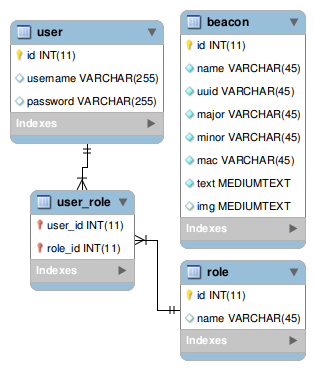
\includegraphics[width=7cm]{./figs/mer.png}
  \caption{Modelo Entidade Relacionamento}
  \par\makebox[\width]{Fonte: Autores}
\end{figure}

A tabela beacon armazena os dados dos \textit{beacons} que são cadastrados pelo sistema de cadastramento e possui as seguintes colunas:

\textbf{Id}: É o identificador único de cada registro na tabela e é constituído por um inteiro que é incrementado automaticamente a cada novo registro.

\textbf{Nome}: Identificação de nome para o
\textit{beacon}.

\textbf{Uuid}: Identificador alfa-numérico.

\textbf{Major}: Número entre 0 e 65523 para identificar com maior precisão um pequeno grupo de \textit{beacons}.

\textbf{Minor}: Número entre 0 e 65523 para identificar com maior precisão um único \textit{beacon}.

\textbf{Mac}: Endereço físico único de cada \textit{beacon}.

\textbf{Texto}: Texto que será exibido no aplicativo.

\textbf{Img}: Imagem convertida em Base64 que será exibida no aplicativo.

A tabela user foi criada para que sejam armazenados os dados de usuários, tais como:

\textbf{Id}: É o identificador único de cada registro na tabela e é constituído por um inteiro que é incrementado automaticamente a cada novo registro.

\textbf{Username}: É o nome que o usuário utilizará para entrar no sistema de cadastramento.

\textbf{Password}: É a senha, criptografada nesta coluna, que será utilizada para que o usuário entre no sistema de cadastramento.

A tabela role armazena as informações referentes a permissão do usuário no sistema, sendo que podem ser cadastrados diferentes perfis para determinadas rotas do sistema. O padrão utilizado é o de administrador. Ela possui os seguintes campos:

\textbf{Id}: É o identificador único de cada registro na tabela e é constituído por um inteiro que é incrementado automaticamente a cada novo registro.

\textbf{Name}: É um nome para identificar o tipo de permissão.

A tabela user\_role é o relacionamento muitos para muitos entre as tabelas user e role. Ela é responsável por ligar um usuário a uma permissão e possui os seguintes campos: 

\textbf{User\_id}: Identificador único da tabela user.

\textbf{Role\_id}: Identificador único da tabela role.